\documentclass[a4paper,11pt]{article} 
\usepackage{listings}
\usepackage{url}
\usepackage{hyperref}
\usepackage{graphicx}
\usepackage{amssymb}					
\usepackage{marvosym}
\usepackage[latin1]{inputenc}    
\usepackage[french]{babel}
\usepackage[T1]{fontenc}
\usepackage{pstricks}
\usepackage{colortbl}
\usepackage{fancybox}
\usepackage{enumerate}
\usepackage{tablists}
\usepackage[dvips]{epsfig}
\usepackage{makeidx}
\usepackage{amsmath,amssymb}
\usepackage{stmaryrd}
\usepackage{xspace}
\usepackage{float}
\usepackage{url}
\usepackage{multicol}
\usepackage{boxedminipage}
\usepackage{listings}
\usepackage{aurical}
\usepackage{slashbox}
\usepackage{threeparttable}
\usepackage{fancyhdr}
\usepackage{algorithm,algorithmic}
\usepackage{pstricks,pst-tree}
\pagestyle{empty}               % On ne num�rote pas les pages
\usepackage{vmargin}            % red�finir les marges
\setmarginsrb{2cm}{2cm}{2cm}{2cm}{0cm}{0cm}{0cm}{0cm}
\newcommand{\pascal}{\textsf{Pascal}\xspace}
\usepackage{pifont}
\usepackage[french]{minitoc}
\catcode`\�=\active
\catcode`\�=\active
\def�{\og\ignorespaces}
\def�{{\fg}}	
\usepackage{color}
\usepackage{lastpage}
\usepackage{wasysym}
\usepackage{tikz-qtree}
\pagestyle{fancy}
\renewcommand{\headrulewidth}{0pt}
\fancyfoot[c]{}
%\fancyfoot[L]{\Letter\  \texttt{\url{Mohamed.Messabihi@gmail.com}}}
\fancyhead[L]{}
\fancyhead[R]{}
%\fancyhead[L]{\sectionname}
%\pagestyle{fancy}
\usepackage{epsdice}
\usepackage{ifsym}
\setcounter{tocdepth}{1}
\renewcommand \thesection  {}
\usepackage{filecontents}
\newcommand{\solution}{\begin{center} \colorbox{yellow}{\large {\textbf{Solution}}}\end{center}}
\lstset{language=C,numbers=left,  numbersep=5pt,framexleftmargin=5mm, %frameround=fttt, 
frame=trBL, %stepnumber=2 rulesepcolor=\color{gray},% backgroundcolor=\color{fondalgo},
belowcaptionskip=1\baselineskip,   breaklines=true,   %frame=L,   xleftmargin=\parindent,
  language=C,   showstringspaces=false,   basicstyle=\footnotesize\ttfamily,   keywordstyle=\bfseries\color{green!40!black},   commentstyle=\itshape\color{purple!40!black},
  identifierstyle=\color{blue},   commentstyle=\color{gray},   stringstyle=\color{red} ,
  %caption={Programme Myst�re},   label=evaluation,  
  } 

%#######################################################################################


\begin{document}
\parbox{\textwidth}{ \small \rule{\textwidth}{1.5pt} \begin{minipage}{.5\textwidth}
\begin{flushleft} \textbf{Auteur} : Mohamed Messabihi\\   \textbf{Mati�re} : Programmation et structures de donn�es\\  \textbf{Date}  18 Mai 2017 \\ \textbf{Dur�e}  1h30 \\ \end{flushleft}
\end{minipage} 
 \hfill \begin{minipage}{.08\textwidth} \begin{center}
\includegraphics[width=1cm]{logo.jpg}\end{center} \end{minipage} \hfill \begin{minipage}{.4\textwidth} \begin{flushright} Universit� Abou Bakr Belka�d - Tlemcen\\ Facult� des Sciences \\1\up{�re} Ann�e MI \\ Semestre 2 \end{flushright} \end{minipage} \rule {\textwidth}{1.5pt}}
%################################################################################
\pagenumbering{arabic} \setcounter{page}{1}
\begin{center}
\section*{Examen final}
\rule{.7\textwidth}{.5pt}\\
\footnotesize{{\textsf {Aucun document n'est autoris�\\
Les solutions doivent �tre r�dig�es en \textbf{C} \\
Les appareils portables doivent �tre  �teints et pos�s sur le bureau du surveillant}}}
\rule{.7\textwidth}{.5pt}
\end{center}
 
\section{Affichage \hfill 2 pts.  \Clocklogo 15' }
\input{Supprimer-Occ}
\section{Allers-retours \hfill 7 pts.  \Clocklogo 25'}
%\section{Allers-retours \hfill 8 pts.  \Clocklogo 30'}
�crire une fonction qui transforme un tableau \textsf{TAB} de deux dimension (\textsf{N} lignes et \textsf{M} colonnes) en un tableau lin�aire A (� une seule dimension \textsf{L}). La fonction affecte les valeurs dans le tableau lin�aire \textsf{A} en  parcourant en allers-retours le tableau � deux dimensions \textsf{TAB}. Autrement dit, la fonction  parcourra la premi�re ligne de \textsf{TAB} de gauche � droite puis la seconde de droite � gauche, la troisi�me  de gauche � droite et ainsi de suite en alternant, � chaque fois,  le sens de parcours des lignes.

%\vspace{5mm}
\textbf{Exemple :}
\vspace{-5mm}
\begin{center}
%\begin{tabular}{|c|c|c|c|}
%\hline 
%\rule[-1ex]{0pt}{2.5ex} 11 & 2 & 8 & 4 \\ 
%\hline 
%\rule[-1ex]{0pt}{2.5ex} 19 & 7 & 13 & 9 \\ 
%\hline 
%\rule[-1ex]{0pt}{2.5ex} 6 & 14 & 10 & 3 \\ 
%\hline 
%\rule[-1ex]{0pt}{2.5ex} 16 & 1 & 12 & 5 \\ 
%\hline 
%\rule[-1ex]{0pt}{2.5ex} 18 & 17 & 20 & 15 \\ 
%\hline 
%\end{tabular} 
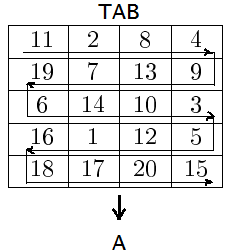
\includegraphics[scale=.6]{Allers-retours.png} 
\end{center}
 
 \vspace{-6mm}
\begin{center}
\begin{tabular}{|c|c|c|c|c|c|c|c|c|c|c|c|c|c|c|c|c|c|c|c|}
\hline 
 11 & 2 & 8 & 4 & 9 & 13 & 7 & 19 & 14 & 6 & 10 & 3 & 5 & 12 & 1 & 16 & 18 & 17 & 20 & 15 \\ 
\hline 
\end{tabular} 
  \end{center}
  %\textbf{  Attention : } il ne faut pas utiliser un autre  tableau interm�diaire 

\endinput
\solution
\begin{center}
\begin{minipage}{.7\textwidth}
 %footnotesize
  \lstinputlisting{Allers-retours.c}
%[firstline=1,lastline=10]
 \end{minipage}
 \end{center}
\section{Rectangles \hfill 11 pts.  \Clocklogo 50'}
%\section{Rectangles \hfill 11 pts.  \Clocklogo 50'}

On souhaite programmer un �diteur graphique qui permet de dessiner des rectangles sur un plan muni d'un rep�re cart�sien.

Un rectangle est d�fini par :
\begin{itemize}
\item un \textsf{point} sur le plan qui repr�sente son coin sup�rieur gauche ;
\item une \textsf{longueur} ;
\item une \textsf{largeur} ;
\item et une \textsf{couleur} qui peut �tre  blanche, noire ou grise.
\end{itemize} 

 Un point \textsf{P}  est d�fini par un couple de r�els :
 \begin{itemize}
 \item  \textsf{x} appel� l'abscisse de \textsf{P} ;
\item   \textsf{y} appel� l'ordonn�e de \textsf{P}.
 \end{itemize}


\begin{enumerate}
%\vspace{.25cm}
\item D�finir la structure {\textsf{Rectangle}}.  \hfill  \textbf{3 pts} 


%\vspace{.25cm}
\item \'Ecrire une fonction {\textsf{saisir\_Rectangle}}. \hfill \textbf{2 pts} 

%\vspace{.25cm}
\item  \'Ecrire une fonction {\textsf{deplacer}} qui prend en entr�e un rectangle R et un point P$\prime$ et puis elle d�place le rectangle R vers le point P$\prime$. Par exemple, le rectangle R1, de la figure ci-dessous, prendra la place du rectangle R2 s'il est  d�plac�  au point P'.   \hfill \textbf{1 pt} 


%\vspace{.25cm}
\item  \'Ecrire une fonction {\textsf{zoomer}} qui prend en entr�e un rectangle et un coefficient de zoom. La fonction maintient le coin sup�rieur gauche du rectangle  puis elle agrandie ou elle rapetisse les dimensions du rectangle en fonction du coefficient de zoom.    Par exemple, le rectangle R3 devient �gale au rectangle R4 s'il est zoom�  avec un coefficient �gale � 2 et inversement R4 devient �gale � R3 s'il est zoom�  avec un coefficient �gale � 0.5. \hfill \textbf{1 pt} 

%\vspace{.25cm}
\item  \'Ecrire une fonction {\textsf{sym�trique}} qui prend en entr�e
 un rectangle R et  retourne le rectangle sym�trique 	 R$\prime$  du R par 	rapport � son coin sup�rieur gauche. Par exemple, le rectangle R5 est le r�sultat de l'appel de cette fonction avec le rectangle R4 comme param�tre. \hfill  \textbf{1 pt}   

%\vspace{.25cm}
%\item  \'Ecrire une fonction {\textsf{centre}} qui prend en entr�e un rectangle R et retourne le point qui se trouve � son plein milieu.  \textbf{1 pt} 



%\vspace{.25cm}
\item  \'Ecrire une fonction {\textsf{inclut}} qui prend en entr�e deux  rectangles R1 et R2   et renvoie 1 si R2 est totalement  inclus dans R1, 0 sinon. Par exemple R6 est inclus dans R7 mais R8 ne l'est pas. \hfill \textbf{2 pts} 


\begin{center}
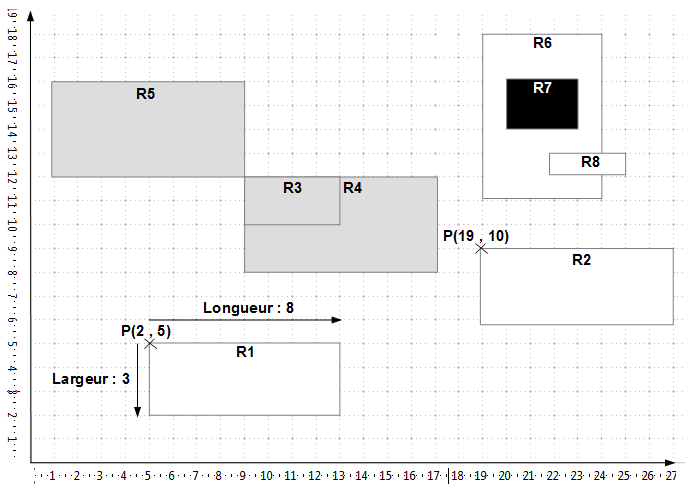
\includegraphics[width = .95\textwidth]{Rectangls.png} 
\end{center}
%\vspace{.25cm}

\item \'Ecrire une fonction \textbf{\textsf{main}} qui permet de : \hfill\textbf{1pt}
\begin{itemize}
\item d�clarer un \textsf{Graph} qui contient un ensemble de rectangles.  
\item saisir le rectangle R1 de la figure ci-dessus dans le premier rectangle de la variable \textsf{Graph}, 
\item d�placer le premier rectangle au point P$\prime(19,9)$, 
\item et enfin,  ajouter  un deuxi�me  rectangle (dans \textsf{Graph}) sym�trique au premier rectangle	 d�plac�.
\end{itemize}  

\end{enumerate}

\endinput

\solution
\begin{center}
\begin{minipage}{.7\textwidth}
 %footnotesize
  \lstinputlisting{Rectangls.c}
%[firstline=1,lastline=10]
 \end{minipage}
 \end{center}



 
\vfill \hfill \emph{ \og Bon courage  \fg}
\end{document}
\endinput